\documentclass[12pt]{article}
\usepackage{listings}
\usepackage[colorlinks=true,pagebackref,linkcolor=blue]{hyperref}
\textwidth=7in
\textheight=9.5in
\topmargin=-1in
\headheight=0in
\headsep=.5in
\hoffset  -.85in

\lstset{
basicstyle=\footnotesize\ttfamily,
language=bash,
upquote=true,
breakatwhitespace=true,
columns=fullflexible,
keepspaces,
%numbers=none,
tabsize=3,
frame=blrt,
framextopmargin=5pt,
showstringspaces=false,
extendedchars=true
}

\pagestyle{empty}

\renewcommand{\thefootnote}{\fnsymbol{footnote}}
\usepackage{graphicx}

\begin{document}



\begin{center}
{\bf AMS 550.400 \quad HW SET 1\quad  Due Date:  Oct 8}\\
\vskip.2in
{\footnotesize Last Compiled on \today}
\end{center}

\setlength{\unitlength}{1in}

\begin{picture}(6,.1) 
\put(0,0) {\line(1,0){6.25}}         
\end{picture}

 

\renewcommand{\arraystretch}{2}

\noindent\textbf{General Instruction:} 
To complete the homework set, you are required to do the followings. 
Your solutions must be typed in \LaTeX\ using the course homework
template.  
The progression of your homework solution is to be
``recorded'' by making a git folder specifically for this homework
set.  The burden of proof is on you, and if your git commit history
is sparse, then you may be liable for a penalty.  
A paper copy of the PDF output of your \LaTeX\ file is 
to be submitted to your instructor in class on the due date.
\emph{After} submitting the paper copy, but \emph{before} the end of
the due date, you will upload your work to your github by making a remote repository
specifically for the homework, and post the link to the repository 
at the designated \emph{Discussion} forum in Blackboard by making 
a thread just for you.  The repository name in your github should be
\texttt{550400.homeworkset.1} and the discussion forum thread should
be named \texttt{YourFirstNameMiddleInitialLastName}, e.g.,
\texttt{BaracHObama} and \texttt{WillardMRommey}. 
You have till the end of 
the due date to finalize your github repository.  
However, any commit made after the class time of the due date will be 
inadmissible. \emph{Your attention to details in following this instruction will be 
critical, and if not followed exactly at the time of collection, the
homework set may be graded at $90\%$ of the full score}.

\vskip.25in
\noindent\textbf{Problem 1 (10 pts):}  
Assume that you are starting from ``scratch'' at the directory \verb+~/+.
Provide a sequence of git/bash commands that yields a git folder with 
a commit history such that:
\begin{itemize}
\item the \emph{master} branch has commits $A$, $B$, $C$, $X$ and $D$,
\item the \emph{alt} branch has commits $A$, $B$, $X$,
\end{itemize}
Suppose that you are currently working on \texttt{master} branch. Draw 
its commit history graph (i.e., the graph portion of the output of
\verb+git log --graph --oneline+).  Next, assume that 
you are on \texttt{alt} branch. Draw its commit history graph.  
 
The following git commands were used for this exercise:

 mkdir Hw1.git\newline
 cd Hw1.git\newline
 git init .\newline
 vi main.txt  (type A)\newline
 git add . \newline
 git commit -m "A" \newline
 vi main.txt  (insert line after A and type "B")
\newline
 git add . \newline
 git commit -m "B"\newline
 git branch alt \newline
 git checkout alt \newline
 vi main.txt ( add line after B and type "X")
\newline
 git add . \newline
 git commit -m "X" \newline
 git checkout master\newline
 vi main.txt (add line after B and type "C")
  \newline
 git add . \newline 
 git commit -m "C" \newline
 git merge alt \newline
 vi main.txt  (resolve conflict)
\newline
 git add .\newline
 git -m "merged" \newline
 vi main.txt (insert line after C and type "D" )
\newline
 git add .
\newline
 git commit -m "D"

\begin{figure}[h]
    \begin{center}
        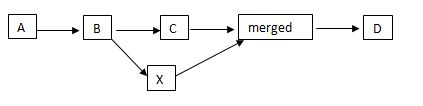
\includegraphics[width=\textwidth]{Hw1Map.jpg}
    \end{center}
    \caption{Master and branch}
    \label{fig:Hw1Map}
\end{figure}

\begin{figure}[h]
    \begin{center}
        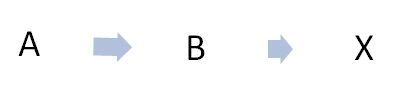
\includegraphics[width=\textwidth]{AltMap.jpg}
    \end{center}
    \caption{Alt Branch}
    \label{fig:Hw1Map}
\end{figure}



\vskip.25in
\noindent\textbf{Problem 2 (10 pts):}
Assume that you are starting from ``scratch'' at the directory \verb+~/+.
Provide a sequence of git/bash commands that yields a git folder and 
\begin{itemize}
\item configure your git with your name and your email address,
\item set up an alias for each of the git remotes listed below:
\begin{verbatim}
git://github.com/nhlee/550400.stanza1.git 
git://github.com/nhlee/550400.stanza2.git 
git://github.com/nhlee/550400.stanza3.git 
\end{verbatim}
Assume that each remote contains exactly single commit with 
a txt file for a single (different) stanza,
\item pull to combine three stanzas of a poem,
\item after the first pull, add the title of the poem,
\item after the second and third pull, resolve the merge conflict,
\item after resolving the third pull merge conflict, push the result
  to your (newly created) remote repository. 
\end{itemize}

The following sequence of git commands was used in this exercise:

mkdir Hw1Prob2.git\newline
 cd Hw1Prob2.git \newline
 git init . \newline
 git remote add stanza1 git://github.com/nhlee/550400.stanza1.git \newline
git pull stanza1 master\newline
vi main.txt (make sure it worked) \newline
git add . \newline
git commit -m "stanza1" \newline
git remote add stanza2 git://github.com/nhlee/550400.stanza2.git\newline
pull stanza2 master\newline
vi main.txt (resolve conflict)\newline
git add . \newline
git commit -m "stanza2 " \newline
git remote add stanza3 git://github.com/nhlee/550400.stanza3.git\newline
git pull stanza3 master\newline
vi main.txt (resolve conflict)\newline
git add .\newline
git commit -m "stanza3" \newline



\newpage
\noindent\textbf{Problem 3 (40 pts):}
Consider a team of four students, say, $A$, $B$, $C$ and $D$, 
who just started working 
on writing a \texttt{latex/beamer} file, say \texttt{main.tex}, 
for a class presentation of their work statement.  
Assume that they do not wish to coordinate their schedules for a
concurrent group meeting (both virtually and physically).  
Assume that:
\begin{itemize}
\item $A$ is in charge of \emph{Introduction},
\item $B$ is of \emph{Problem Statement}, 
\item $C$ is of  \emph{Timeline},
\item $D$ is of \emph{Deliverable} part of the presentation.  
\end{itemize}
In other words, their contributions to \texttt{main.tex} do not overlap.
Then, 
\begin{itemize}
\item first, devise a work flow strategy for the team so that they can
  collaborate asynchronously using \texttt{git},
\item next, devise yet another \texttt{git} strategy different from your earlier
  proposal.  
\end{itemize}
Finally,
\begin{itemize}
\item discuss the strength and weakness of each of your proposed strategies in terms of merge
conflicts resolution,
\item make the final recommendation.  
\end{itemize}
In order to answer this question, \emph{build}
a mathematical model, \emph{following} the guideline from IMM. 
Use Section 1.4 and Section 1.5 of IMM as \emph{role models}.    
For example, you are to identify which variables  are exogenous 
and which are endogenous.  More specifically, among other things, 
in your model, is the preamble part of \texttt{main.tex} an endogenous 
or exogenous variable?  
Note also that in addition to this issue, there are other issues that
you are to consider.  So, \emph{be sure to consult IMM}. 
\paragraph {Proposal 1:}

 In this mechanism each student pushes their files onto their github.com account. Student B pulls from A and Student C pulls from B. Finally, Student D pulls from Student C. This allows for the files to merge without any additional copies being made. In addition, if the specific order is kept then the report will be in order and no further rearrangements will be required. 
\newline 
\newline 
There is much strength to this mechanism. First, when the files are pulled by each student they are in order. Second, the probability of getting extra copies is at a minimum. There are some weaknesses, however. First, each student must be finished with their segment of the report before the next student can pull the file. The fact that the transfer of files must be in that specific order also makes the process less flexible. For example, A must be done before B, B must be done before C and C must be done before D. Another problem occurs with editing. For example, say that A wanted to change something in their section of the report. According to the mechanism, all the students would have to redo the entire process. This takes time and effort.
\newline 
\newline 
To test this we can perform a short simulation. Since I am only one person, it is tedious to establish four new accounts and act as each student. Instead, what I will do is I will use the poem exercise we did in class and act as each student. The first step is to assign a stanza to each student. For example, A will be stanza 1, B will be stanza 2, C will be stanza 3 and D will stanza 4. As B I pull stanza 2 first. I then pull stanza 1 (A) and resolve the conflict. Next, I act as student C so I pull stanza 3. As student C I pull the file from B, which basically contains the file from A and B. As student C, I resolve the conflict. The same applies when I act as student D. We find that the simulation shows that the proposal works, however, it is tedious. 
 

\paragraph {Proposal 2: }
An alternative mechanism is to let each student “submit” their segment to a master directory.  The files are then merged and the conflict is resolved by any one of the students. To do this each student should have a branch. Since Student D is in charge of the “Deliverables” which is usually the last part of the report we will assign student the master directory. This is just case, but it does not have to be this way. If another student volunteers or if the team decides on someone else to be in charge of master directory that will work too. The point is that one person is in charge of resolving the merge conflicts at the end.
\newline 
\newline 
There is much strength to this mechanism. First, only one student will resolve the merge conflicts and compile the documents. This saves time and effort.  Second, the probability of getting extra copies is at a minimum. Third, when it comes to editing it will not be as tedious to recompile and merge again. There are some weaknesses, however.  Because the merge conflicts are managed by one student, there is a chance that if an error occurs there it will not be fixed since there is no proofreading mechanism. Finally, a set deadline must be established or else each student can merge multiple versions which would lead to confusion. 
\newline 
\newline 
To test this we can perform a short simulation. Since I am only one person, what I will do is I will use the poem exercise we did in class and act as each student. The first step is to assign a stanza to each student. For example, A will be stanza 1, B will be stanza 2, C will be stanza 3 and D will stanza 4.  I will first act as student D and create a branches for each student. In each branch I act as each student and pull the stanzas from github. I then checkout and go back to being Student D and pull the last stanza. As student D, I merge all the branches and resolve the conflict. I find that the simulation shows that the proposal works. 

\paragraph {Final Recommendation:} 
My recommedation would go to proposal 2, since it is less tedious and more effiecient.

\vskip0.25in
\noindent\textbf{Problem 4 (aka.\ Fair Play, 40 pts):}
Answer the following question:
\begin{verse}
Is the tennis game fair?
\end{verse}
Note that unlike Problem 3, this question is vaguely stated.
This is intensional, whence to begin, you will first need to clarify
what exactly your question is.
You may use the class discussion on this particular 
problem, but you \emph{may not} directly refer to our 
discussion.  Instead, formulate the model carefully but concisely in 
your own words.   

\vskip0.25in
\noindent\textbf{Final Remarks about Problem 3 \& Problem 4:} 
They are open-ended problems.  However, your scores will be determined
by how well do you follow the exposition style outlined by IMM and
WMA.  For both problems, your write-up should be 
\begin{itemize}
\item self-contained,
\item covering all four parts of Section 1.3 of IMM,
\item paying a particular attention to any causal relation that you
  might be investigating, following Chapter 3 of WMA,
\item answering questions that are explicitly asked in the problem statements.
\end{itemize}
For Problem 3, focus mostly on Step 2 and Step 3 of Section
1.3 of IMM.  For Problem 4, focus mostly on Step 1 and Step
2.  For each problem, minimum 1 pages and maximum 2 pages.
\end{document}
